\documentclass[border=8pt]{standalone}
\usepackage{amsmath,amssymb,bm}
\usepackage{xcolor}
\usepackage{tikz}
\usetikzlibrary{arrows.meta}
\definecolor{ACC}{HTML}{D5772A}
\definecolor{ink}{HTML}{1B1B2F}
\begin{document}
\large
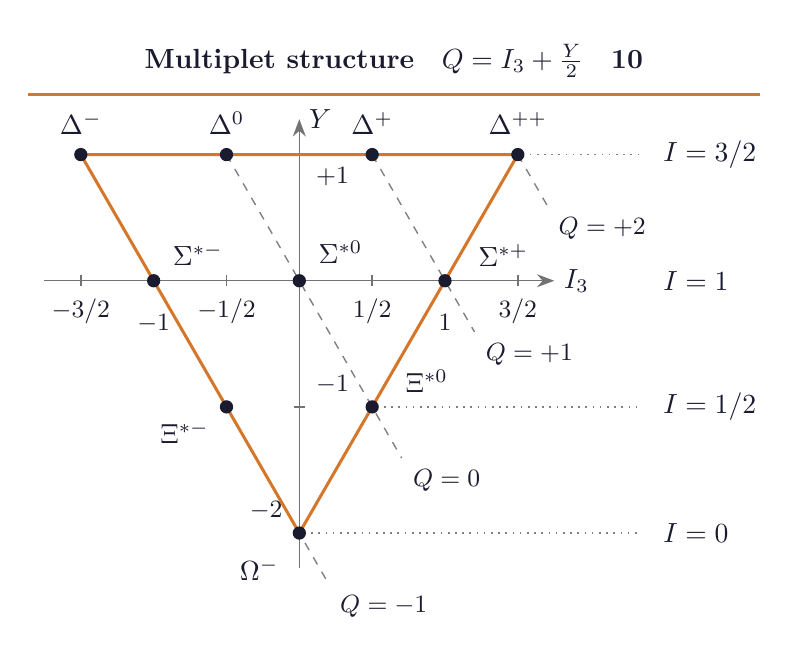
\begin{tikzpicture}[>=Stealth, every node/.style={text=ink}]
\path[use as bounding box] (-3.450,-4.286) rectangle (5.850,3.214);
\node at (1.200,2.789) {\textbf{Multiplet structure}\quad $Q=I_3+\tfrac{Y}{2}$\quad $\mathbf{10}$};
\draw[ACC,line width=.9pt] (-3.450,2.364) -- (5.850,2.364);
\draw[-{Stealth[length=2.2mm]},black!55,line width=.5pt] (-3.238,0) -- (3.238,0) node[right] {$I_3$};
\draw[-{Stealth[length=2.2mm]},black!55,line width=.5pt] (0,-3.654) -- (0,2.052) node[right] {$Y$};
\draw[black!55,line width=.5pt] (-2.775,-0.07) -- (-2.775,0.07); \node[anchor=north,font=\small] at (-2.775,-0.100) {$-3/2$};
\draw[black!55,line width=.5pt] (-1.850,-0.07) -- (-1.850,0.07); \node[anchor=north,font=\small] at (-1.850,-0.300) {$-1$};
\draw[black!55,line width=.5pt] (-0.925,-0.07) -- (-0.925,0.07); \node[anchor=north,font=\small] at (-0.925,-0.100) {$-1/2$};
\draw[black!55,line width=.5pt] (0.925,-0.07) -- (0.925,0.07); \node[anchor=north,font=\small] at (0.925,-0.100) {$1/2$};
\draw[black!55,line width=.5pt] (1.850,-0.07) -- (1.850,0.07); \node[anchor=north,font=\small] at (1.850,-0.300) {$1$};
\draw[black!55,line width=.5pt] (2.775,-0.07) -- (2.775,0.07); \node[anchor=north,font=\small] at (2.775,-0.100) {$3/2$};
\draw[black!55,line width=.5pt] (-0.07,1.602) -- (0.07,1.602); \node[anchor=north west,font=\small] at (0.090,1.562) {$+1$};
\draw[black!55,line width=.5pt] (-0.07,-1.602) -- (0.07,-1.602); \node[anchor=south west,font=\small] at (0.090,-1.562) {$-1$};
\draw[black!55,line width=.5pt] (-0.07,-3.204) -- (0.07,-3.204); \node[anchor=south east,font=\small] at (-0.090,-3.164) {$-2$};
\draw[black!50,dashed,line width=.5pt] (2.775,1.602) -- (3.150,0.952);
\node[anchor=north west,font=\small] at (3.170,0.932) {$Q=+2$};
\draw[black!50,dashed,line width=.5pt] (0.925,1.602) -- (2.225,-0.650);
\node[anchor=north west,font=\small] at (2.245,-0.670) {$Q=+1$};
\draw[black!50,dashed,line width=.5pt] (-0.925,1.602) -- (1.300,-2.252);
\node[anchor=north west,font=\small] at (1.320,-2.272) {$Q=0$};
\draw[black!50,dashed,line width=.5pt] (-2.775,1.602) -- (0.375,-3.854);
\node[anchor=north west,font=\small] at (0.395,-3.874) {$Q=-1$};
\draw[ACC,line width=1.1pt,line join=round] (2.775,1.602) -- (-2.775,1.602) -- (0.000,-3.204) -- cycle;
\fill[ink] (2.775,1.602) circle (2.4pt);
\fill[ink] (0.925,1.602) circle (2.4pt);
\fill[ink] (-0.925,1.602) circle (2.4pt);
\fill[ink] (-2.775,1.602) circle (2.4pt);
\fill[ink] (1.850,0.000) circle (2.4pt);
\fill[ink] (0.000,0.000) circle (2.4pt);
\fill[ink] (-1.850,0.000) circle (2.4pt);
\fill[ink] (0.925,-1.602) circle (2.4pt);
\fill[ink] (-0.925,-1.602) circle (2.4pt);
\fill[ink] (0.000,-3.204) circle (2.4pt);
\node[anchor=south] at (2.775,1.732) {$\Delta^{++}$};
\node[anchor=south] at (0.925,1.732) {$\Delta^{+}$};
\node[anchor=south] at (-0.925,1.732) {$\Delta^{0}$};
\node[anchor=south] at (-2.775,1.732) {$\Delta^{-}$};
\node[anchor=south west] at (-1.730,0.070) {$\Sigma^{*-}$};
\node[anchor=south west] at (0.120,0.100) {$\Sigma^{*0}$};
\node[anchor=south west] at (2.150,0.060) {$\Sigma^{*+}$};
\node[anchor=north east] at (-1.025,-1.662) {$\Xi^{*-}$};
\node[anchor=south west] at (1.225,-1.542) {$\Xi^{*0}$};
\node[anchor=north east] at (-0.140,-3.404) {$\Omega^{-}$};
\draw[black!50,dotted,line width=.6pt] (2.925,1.602) -- (4.350,1.602);
\node[anchor=west] at (4.500,1.602) {$I=3/2$};
\node[anchor=west] at (4.500,0.000) {$I=1$};
\draw[black!50,dotted,line width=.6pt] (1.075,-1.602) -- (4.350,-1.602);
\node[anchor=west] at (4.500,-1.602) {$I=1/2$};
\draw[black!50,dotted,line width=.6pt] (0.150,-3.204) -- (4.350,-3.204);
\node[anchor=west] at (4.500,-3.204) {$I=0$};
\end{tikzpicture}
\end{document}
